\documentclass{report}
\usepackage[latin1]{inputenc}
\usepackage{hyperref}
\usepackage{graphicx}

\title{%
    \begin{minipage}\linewidth
        \centering
        Rapport de projet\\
        \large WEB API REST - Gestion d'une mediath\`{e}que
    \end{minipage}
}

\author{
	\textbf{Marie-Laure FASQUEL} \\
	\'{E}tudiante M1 ISIDis - Universit\'{e} du Littoral C\^{o}te d'Opale\\
	fasquel.ml@gmail.com\\
	\\
	\textbf{K\'{e}vin VASSEUR} \\
	\'{E}tudiant M1 ISIDis - Universit\'{e} du Littoral C\^{o}te d'Opale\\
	vasseur.isn@gmail.com\\
}
\date{\textbf{\today}}


\begin{document}
	\maketitle
	\begin{abstract}
		Le but de ce projet est de cr\'{e}er une WEB API REST qui g\`{e}re une mediath\`{e}que. La date de lancement de ce projet est dat\'{e} au 13 mars 2017 et sa date de livraison est fix\'{e}e au samedi 1 avril 2017. Nous avons libre choix dans les technologies employ\'{e}es. \\
	\end{abstract}
	
	\tableofcontents	
	
	\chapter{Pr\'{e}sentation}
	% ########## TECHNOS ##########
	
	\section{Technologies}
		\subsection{Technologies utilis\'{e}es}
			\subsubsection{Environnement WAMP}
			\textbf{Version :} 3.0.6 \\
			\begin{itemize}
			\item PHP : 5.6.25
			\item MySQL : 5.7.14
			\item Apache : 2.4.23
			\end{itemize}
			
			\subsubsection{Cake PHP}
			\textbf{Version :} 2.9.9 (au lieu de la 3.4.3) \\
			Comme la structure de la version 3 n'est plus la m\^{e}me que celle de la version 2, nous sommes retourn\'{e}s vers celle ci car c'est celle que K\'{e}vin VASSEUR maitrise le mieux.
			\subsubsection{Bootstrap}
			\textbf{Version :} 3 \\		
			
		\subsection{Niveau des membres (avant projet)}
			\subsubsection{Marie-Laure FASQUEL}
			\textit{"J'ai d\'{e}j\`{a} utilis\'{e} Bootstrap, git et l'environnement WAMP dans d'autres projets. Je n'ai par contre jamais manipuler CakePHP."}
			\subsubsection{K\'{e}vin VASSEUR}
			\textit{"Chaque technologies utilis\'{e}es dans ce projet ne me sont pas inconnue. Ce projet me permettra donc d'approfondir encore un peu plus mon exp\'{e}rience."}
			
	% ########## CONSIGNES ##########		
	\section{Consignes}
	\begin{enumerate}
		\item \textbf{/books} - \textit{donne la liste des livres (m\'{e}thode Get)}
		\item \textbf{/books} - \textit{cr\'{e}e un livre dans la base (m\'{e}thode Post)}
		\item \textbf{/books/[int]} - \textit{donne le livre \`{a} l'identifiant donn\'{e} (m\'{e}thode Get)} 
		\item \textbf{/books/[int]} - \textit{supprime un livre dans la base (m\'{e}thode Delete)} 
		\item \textbf{/books/[int]} - \textit{met \`{a} jour un livre dans la base (m\'{e}thode Put}) 
		\item \textbf{/members/[int]/books} - \textit{affiche les livres pour le membre donn\'{e} (m\'{e}thode Get)} 
	\end{enumerate}
	
	
	\section{R\'{e}sultats en utilisant PostMan}
		\subsection{Question 1}
		\begin{center}
			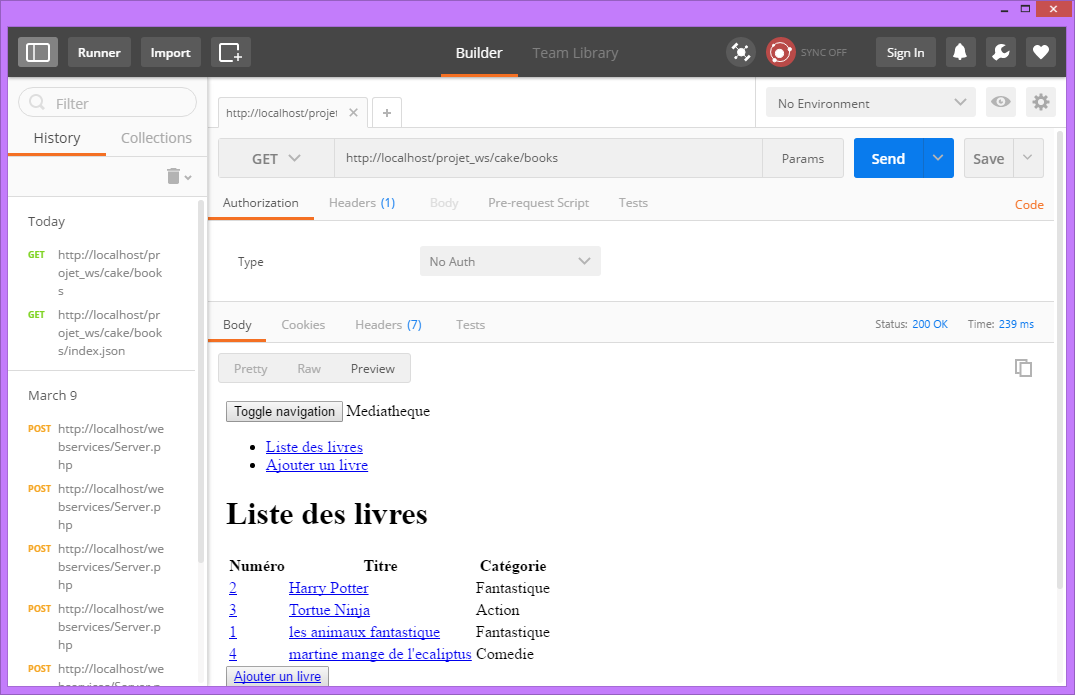
\includegraphics[scale=0.4]{img/resultats/q1,1.png} 
		\end{center} 
		\begin{center}
			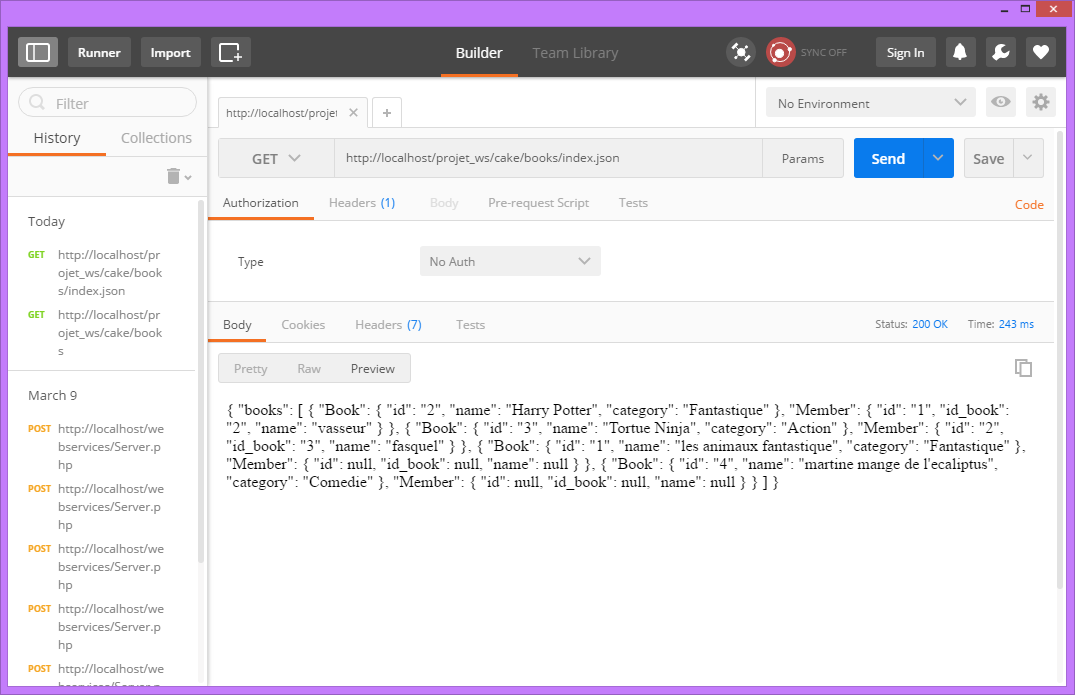
\includegraphics[scale=0.4]{img/resultats/q1,2.png} 
		\end{center}
		\subsection{Question 2}
		La m\'{e}thode POST n'\'{e}tant activ\'{e}e que par le bouton du formulaire, nous ne pouvons pas d\'{e}montrer le r\'{e}sultat de l'URL par PostMan mais en r\'{e}alisant un inspection de la page.
		\begin{center}
			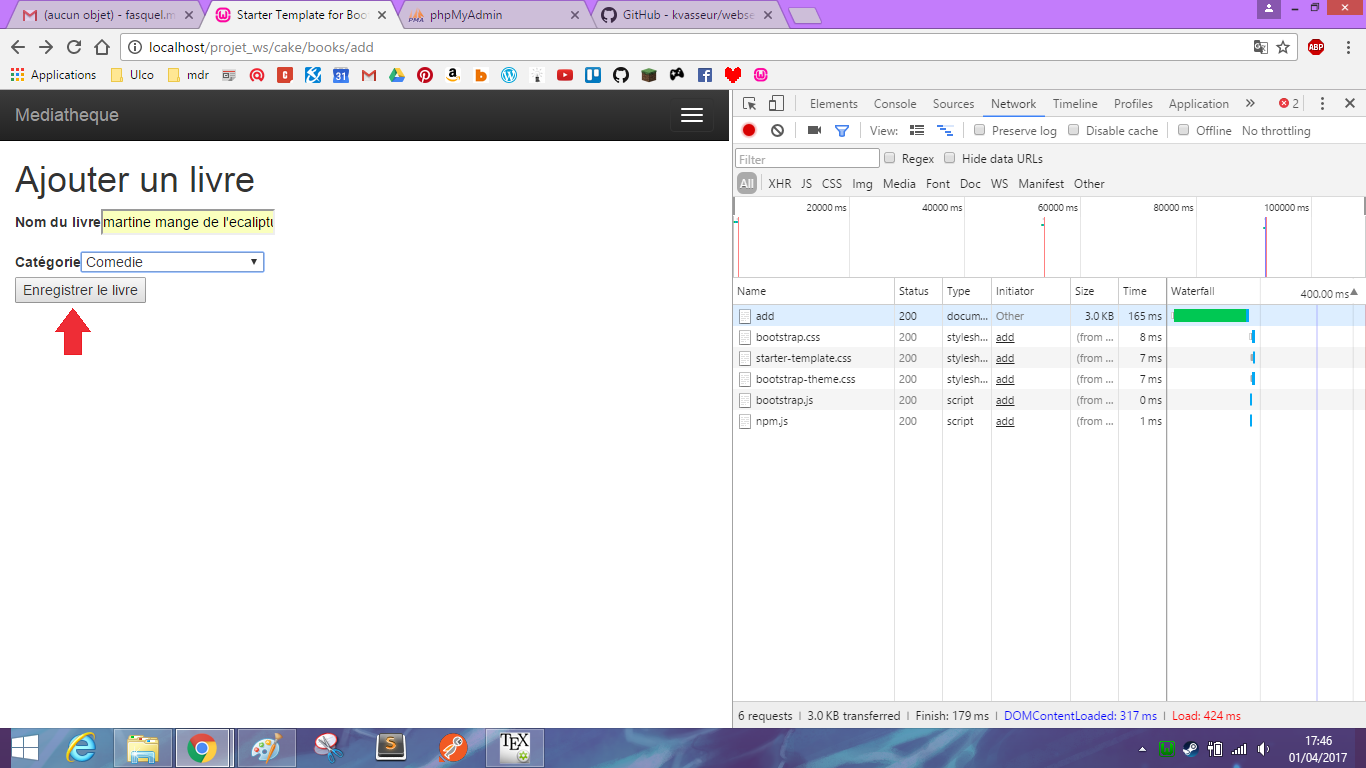
\includegraphics[scale=0.4]{img/resultats/q2,1.png} 
		\end{center} 
		\begin{center}
			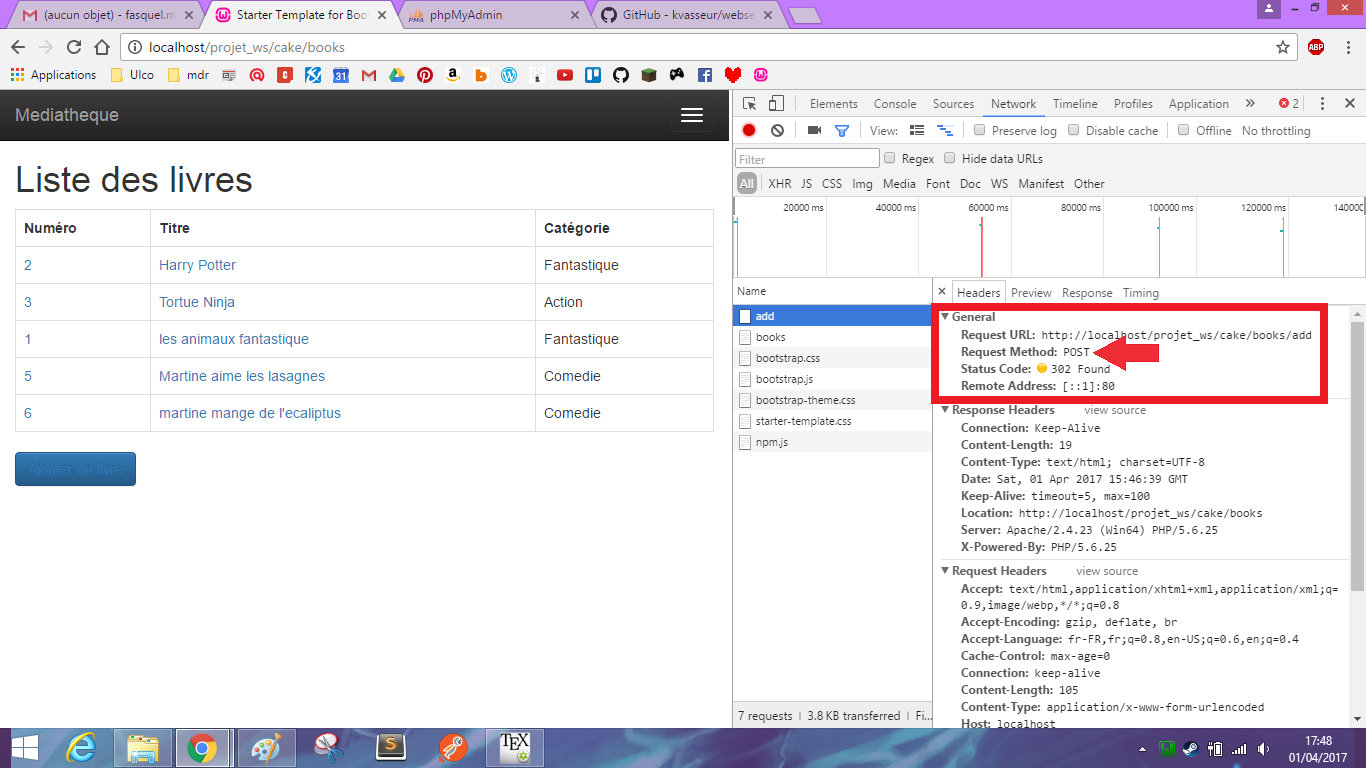
\includegraphics[scale=0.4]{img/resultats/q2,2.png} 
		\end{center}	
		\subsection{Question 3}
		\begin{center}
			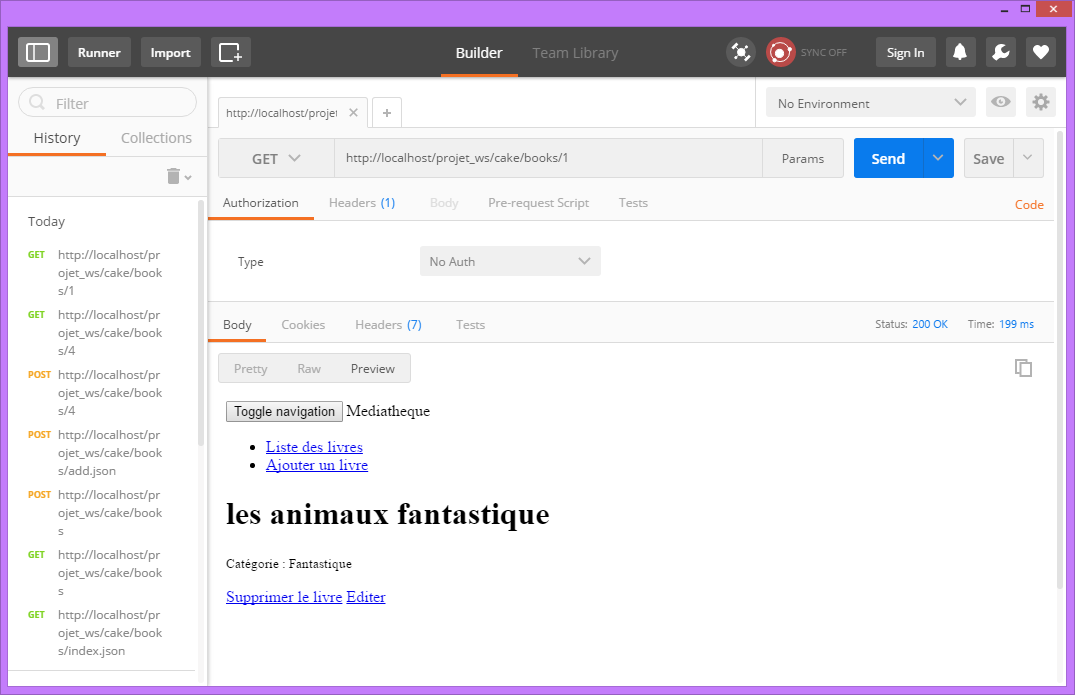
\includegraphics[scale=0.4]{img/resultats/q3.png} 
		\end{center} 
		\subsection{Question 4}
		\begin{center}
			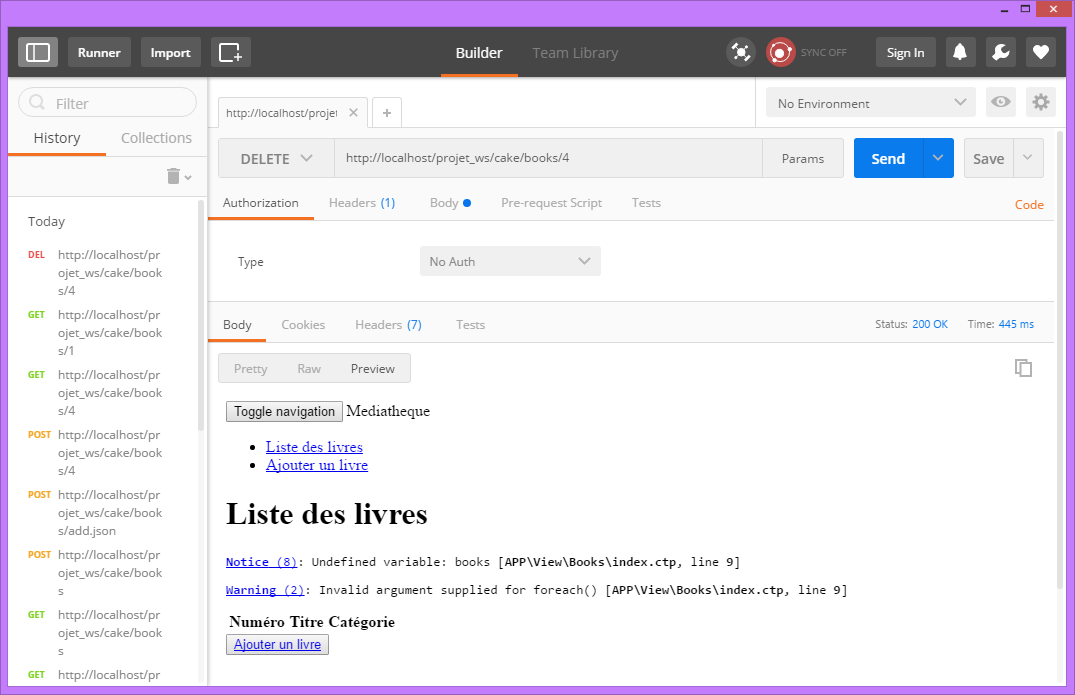
\includegraphics[scale=0.4]{img/resultats/q4,1.png} 
		\end{center} 
		\begin{center}
			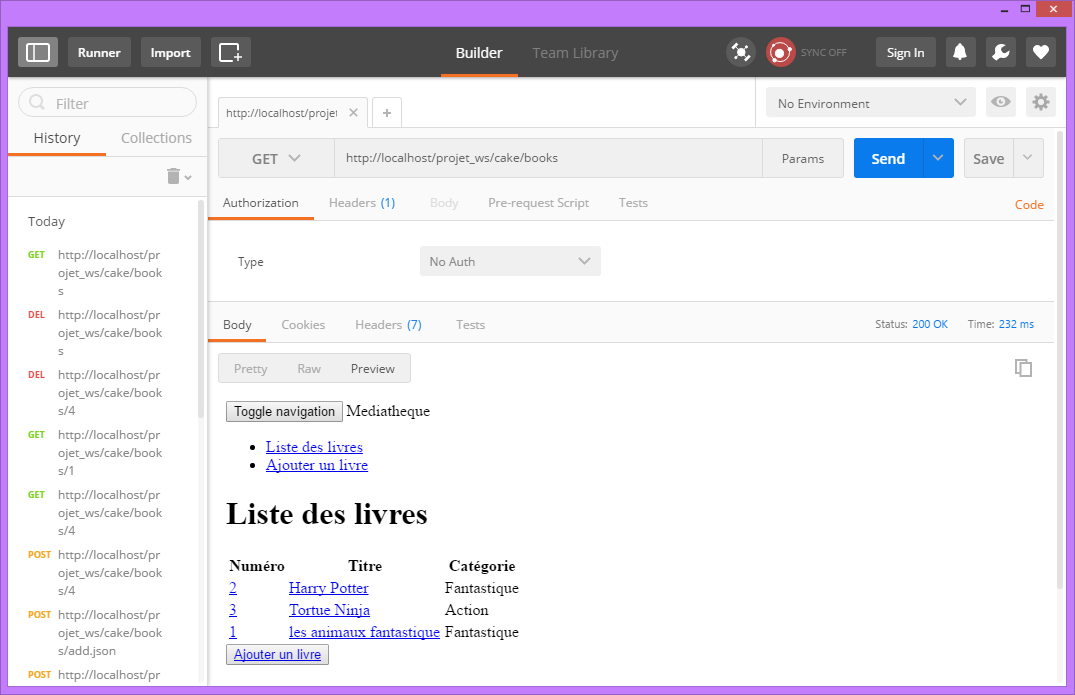
\includegraphics[scale=0.4]{img/resultats/q4,2.png} 
		\end{center}
		\subsection{Question 5}
		\begin{center}
			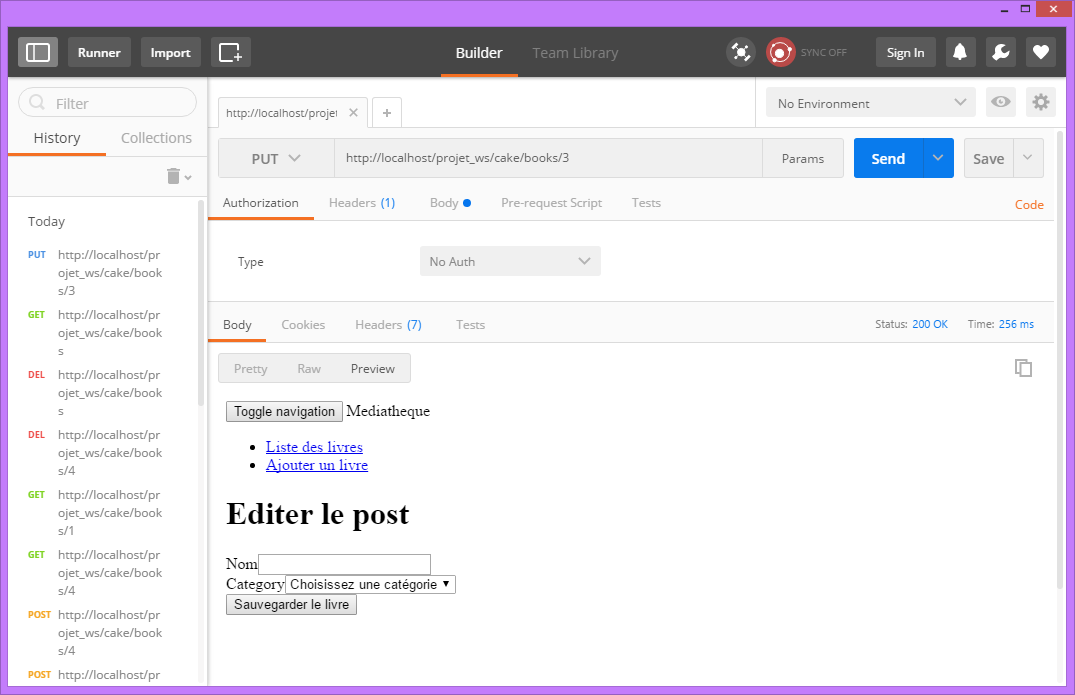
\includegraphics[scale=0.4]{img/resultats/q5.png} 
		\end{center} 
		\subsection{Question 6}
		\begin{center}
			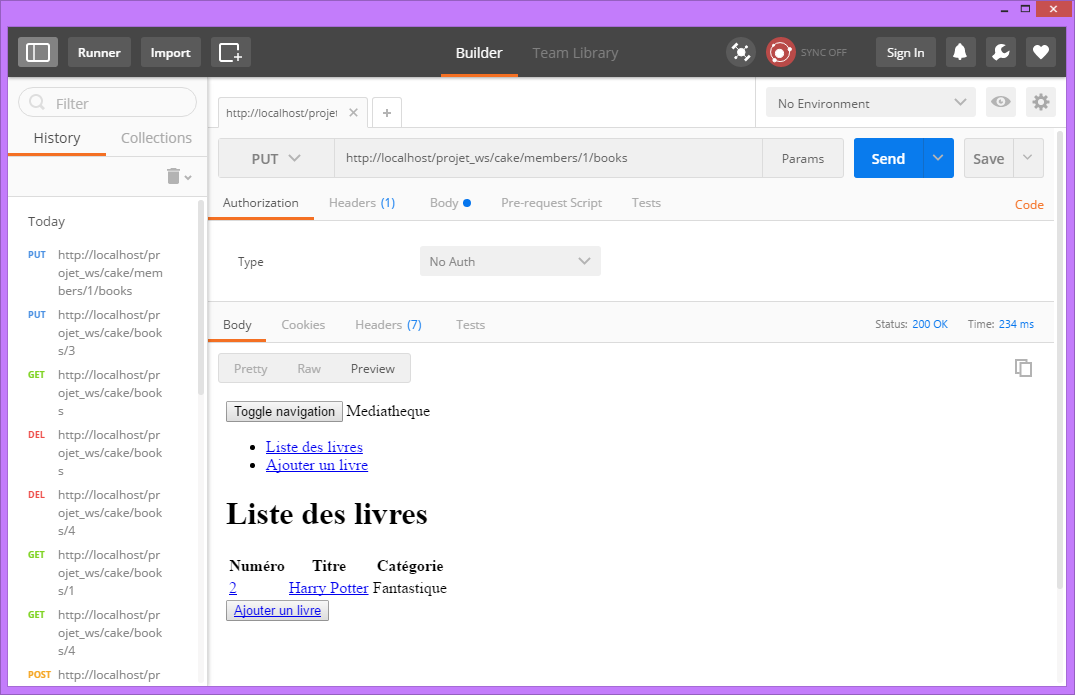
\includegraphics[scale=0.4]{img/resultats/q6.png} 
		\end{center} 
		
	\section{Liens}
		\href{https://github.com/kvasseur/webservices}{Github} \\
		\href{https://trello.com/b/A1vuuQZb/webservices-api-rest-mediatheque}{Trello}
	
	
	% ########## DOCUMENTATION ##########	
	\chapter{Manuel d'installation}
	
	\begin{enumerate}
		\item Si vous ne poss\'{e}dez pas l'environnement WAMP, vous pouvez la t\'{e}l\'{e}charger sur le site officiel : \href{http://www.wampserver.com/}{WAMP}\\
		Un tutoriel d'installation est disponible sur ce site: \href{http://www.cndp.fr/crdp-dijon/Installer-et-configurer-Wampserver.html}{lien}
		\item Allez sur le site : \url{https://github.com/kvasseur/webservices}
		\item Cliquez sur "Clone or download" puis sur "Download ZIP"
		\item Renommez \textit{"webservices-master"} en \textit{"webservices"}
		\item Mettre le fichier \textit{"webservices"} dans le fichier \textit{"www"} (chemin : C:\textbackslash wamp\textbackslash www)
		\item Acc\'{e}der au site avec le lien: \url{http://localhost/webservices/cake/books}
	\end{enumerate}
	
	\begin{center}
	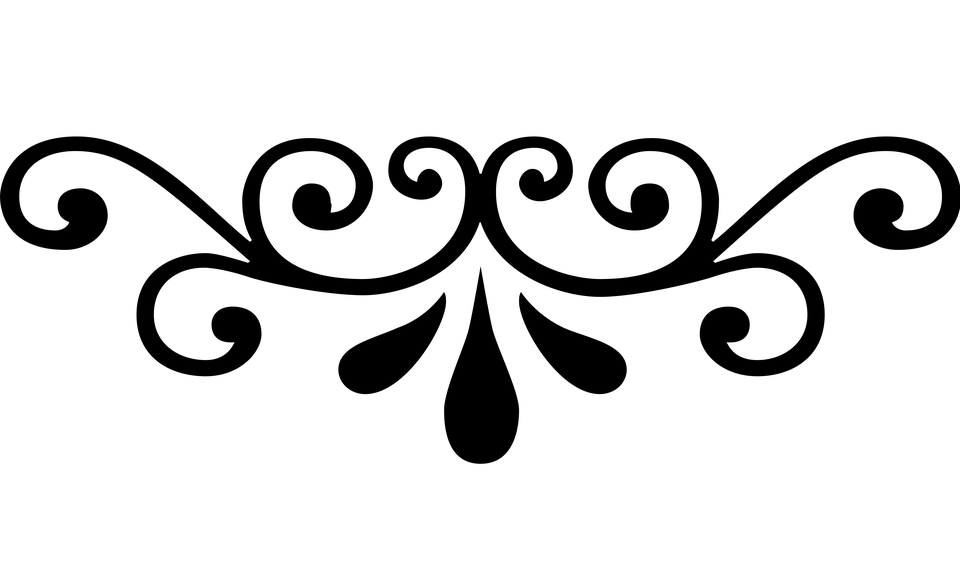
\includegraphics[scale=0.1]{img/fioritures.png} 
	\end{center} 
	
	\chapter{Manuel d'utilisation}
		\section{Menu}
		\begin{center}
			
\includegraphics[scale=0.4]{img/manuel/menu.png}  
		\end{center}
		Via ce menu, vous pouvez soit:
		\begin{itemize}
		\item Acc\'{e}der \`{a} la page de la liste des livres
		\item Acc\'{e}der \`{a} la page d'ajout de livres
		\end{itemize}
		 
		\section{Liste des Livres}
		La page \textit{"Liste des Livres"} (qui est aussi la page d'accueil) renvoi vers la liste des livres.	
		\begin{center}
			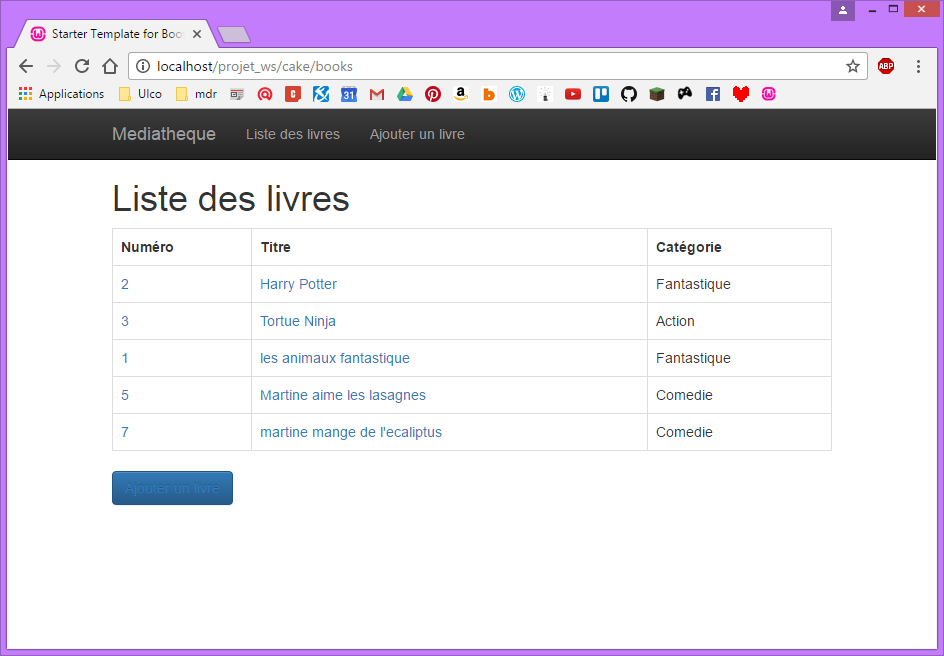
\includegraphics[scale=0.4]{img/manuel/ListeDesLivres.png}  
		\end{center}
		
			\subsection{D\'{e}tails sur un Livre}
			Pour acc\'{e}der au d\'{e}tails d'un livre, cliquez sur le titre ou le num\'{e}ro du livre souhait\'{e}.
			\begin{center}
				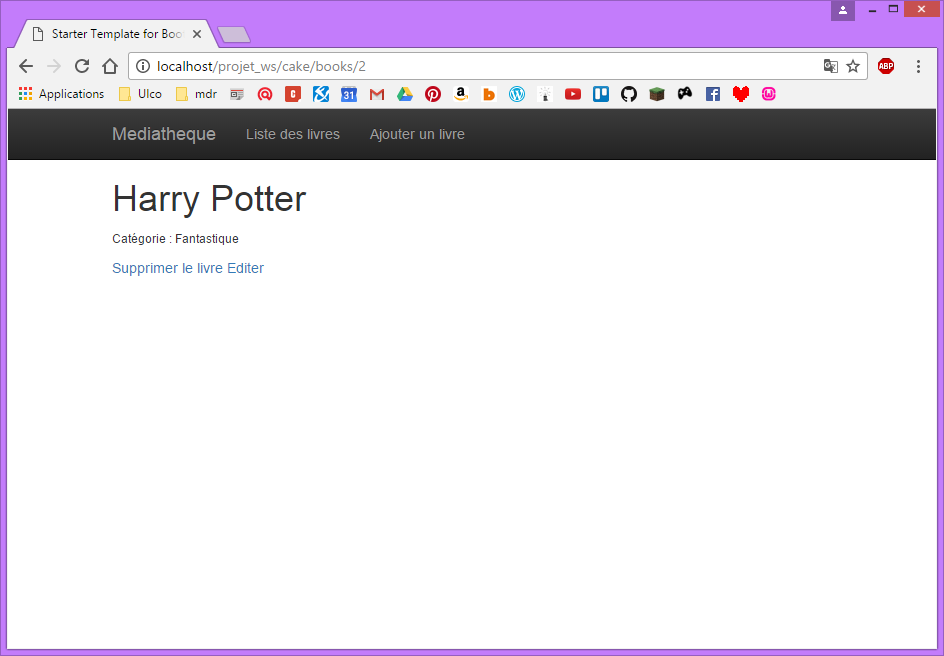
\includegraphics[scale=0.4]{img/manuel/DetailLivre.png}  
			\end{center}
			
			\subsection{D\'{e}tails sur un Livre - Supprimer}
			Lorsque vous cliquez sur \textit{"Supprimer"} sur la page de \textit{"d\'{e}tail du livre"}, un message d'alerte vous demande si vous souhaitez r\'{e}element r\'{e}aliser cette action.
			\begin{center}
				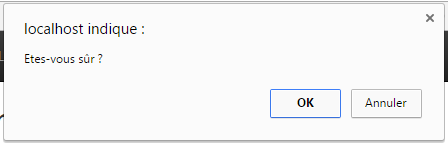
\includegraphics[scale=0.4]{img/manuel/DetailLivre_Supprimer.png}  
			\end{center}
			\textbf{Si vous cliquez sur \textit{"Annuler"}}, le livre ne sera pas supprimer et vous resterez sur la page du \textit{"d\'{e}tail du livre"}.\\
			\textbf{Si vous cliquez sur \textit{"OK"}}: 
			\begin{itemize}
			 \item \textbf{Si le livre n'appartient \`{a} personne}: le livre sera supprim\'{e} et vous aurez une redirection vers la page \textit{"Liste des Livres"} qui sera ainsi mise \`{a} jour. 
			 \item \textbf{Si le livre appartient \`{a} une personne}: le livre ne sera pas supprim\'{e} et vous aurez un message d'erreur : 
			\end{itemize} 
			
			\begin{center}
				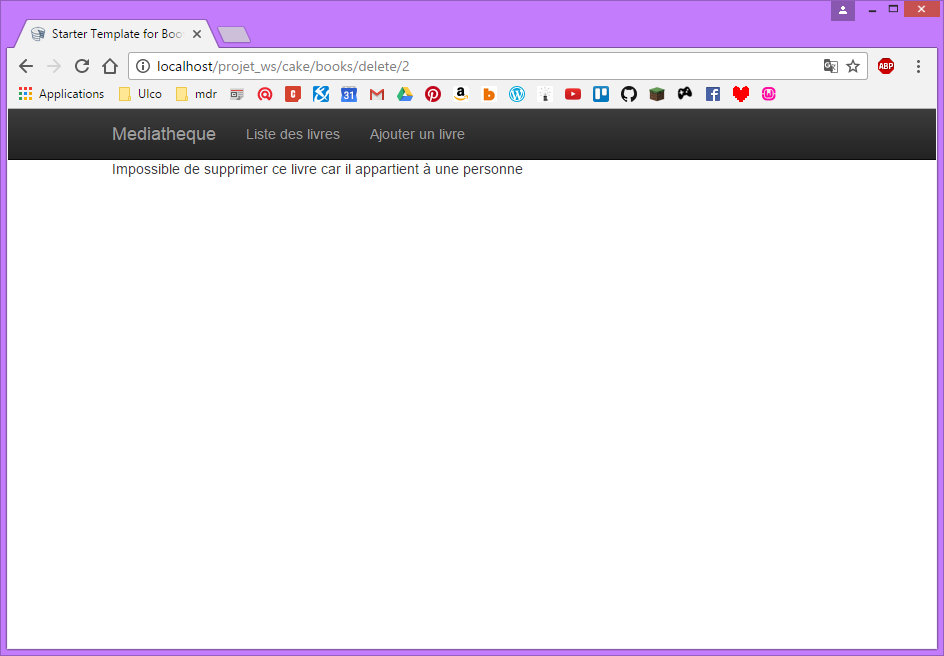
\includegraphics[scale=0.4]{img/manuel/DetailLivre_Supprimer_error.png}  
			\end{center}
			
			\subsection{D\'{e}tails sur un Livre - \'{E}diter}
			Lorsque vous cliquez sur \textit{"\'{E}diter"} sur la page de d\'{e}tail du livre, vous \'{e}tes redirig\'{e} sur la page d'\'{e}dition de ce livre. Ainsi, vous pourrez modifier son titre ainsi que sa cat\'{e}gorie.
			\begin{center}
				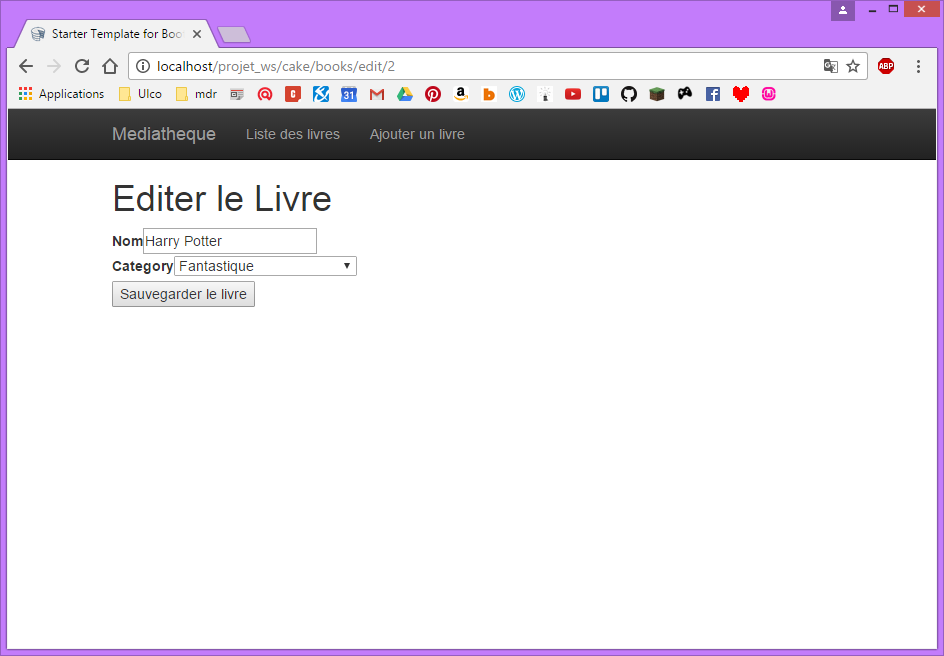
\includegraphics[scale=0.4]{img/manuel/DetailLivre_Editer.png}  
			\end{center}
			
		\section{Ajouter un Livre}
		La page \textit{"Ajouter un Livre"} permet d'ajouter de nouveaux livres en y indiquant le titre ainsi que sa cat\'{e}gorie.
		\begin{center}
			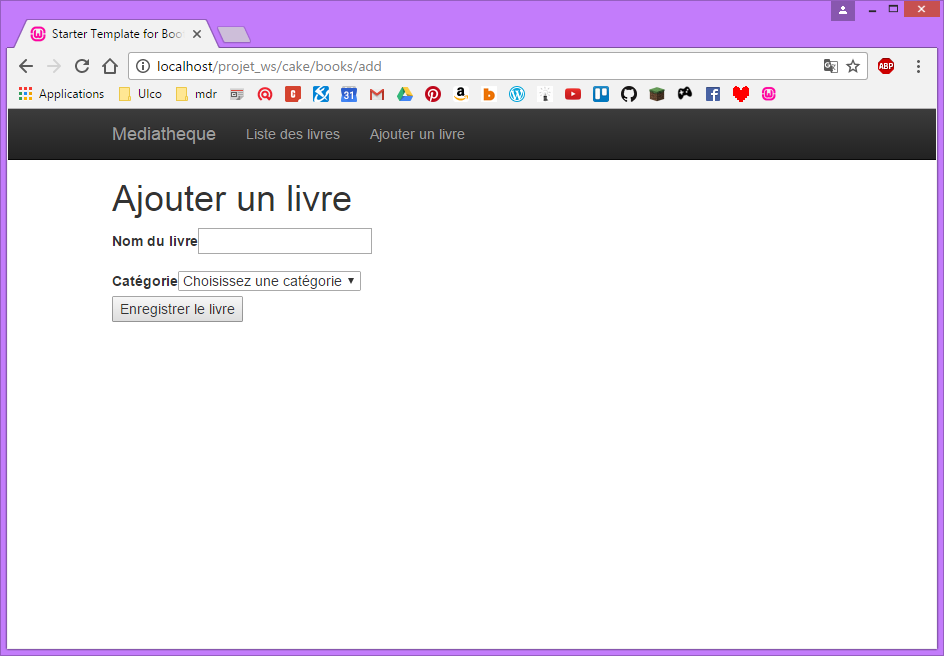
\includegraphics[scale=0.4]{img/manuel/DetailAjouterLivre.png}  
		\end{center}
		
		D\'{e}s que vous cliquez sur \textit{"Enregistrer le livre"}, le livre sera ajout\'{e} et vous aurez une redirection vers la page \textit{"Liste des Livres"} qui sera ainsi mise \`{a} jour.
		
		\begin{center}
		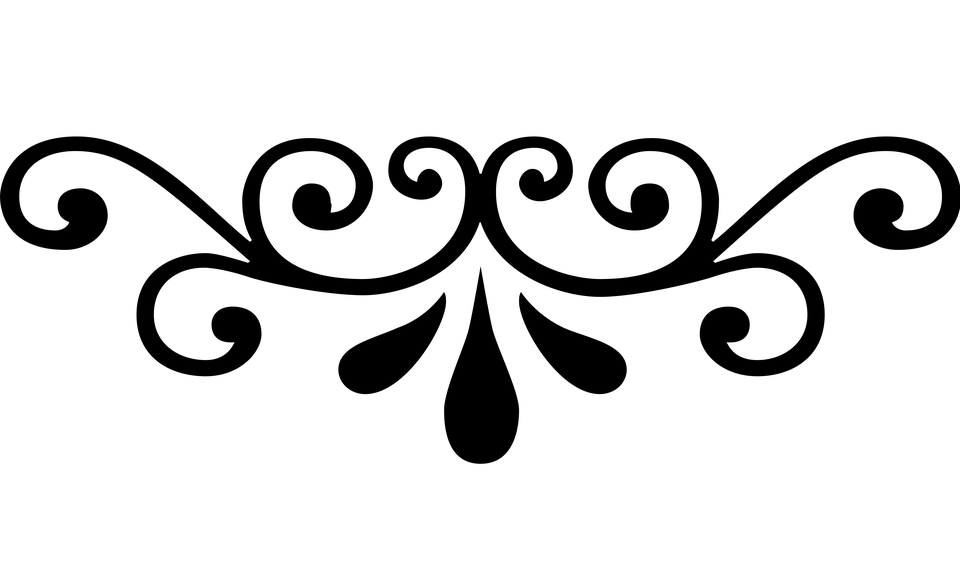
\includegraphics[scale=0.1]{img/fioritures.png} 
		\end{center} 
	
\end{document}